\chapter{Results and Discussion/Analysis}
\label{ch:results}

\section{Experimental Setup and Verification Framework}
\label{sec:exp_setup}
All experiments, cipher models, and fault simulators were verified in Python 3.12, validated against known-answer test vectors, and executed in RARS 1.6 across hundreds of randomized Monte Carlo trials.

\section{Cryptographic Test Vector Validation}
\label{sec:test_vectors}
Both cipher implementations were validated against canonical test vectors:
\begin{itemize}
    \item \textbf{BAKSHEESH}: Validated against all 8 official test vectors from Table 14 of Baksi et al.~\cite{baksi2023baksheesh} $\to$ \textbf{8/8 PASS (100\% Compliant)}.
    \item \textbf{GIFT-128}: Validated against the CHES 2017 canonical all-zero vector plus two independent reference vectors $\to$ \textbf{3/3 PASS (100\% Compliant)}.
\end{itemize}

\section{Empirical LDFA Attack Results on BAKSHEESH}
\label{sec:exp_ldfa}
On unprotected implementations, LDFA was evaluated across 25 independent random keys:
\begin{itemize}
    \item Exactly \textbf{31 faulty ciphertexts} were required per key recovery.
    \item The candidate key space collapsed to exactly \textbf{16 candidates ($2^4$)} in every trial.
    \item Disambiguation using 1 known $(P, C)$ pair achieved \textbf{100\% success rate} (25/25 trials).
    \item Mean key recovery execution time: \textbf{0.024 seconds}.
\end{itemize}

\section{Empirical LIFA Attack Results under Active Redundancy}
\label{sec:exp_lifa}
When duplicate-and-compare redundancy is active, effective faults are suppressed. Over 12,723 queries across 25 trials:
\begin{itemize}
    \item \textbf{Observed Ineffectiveness Rate}: $6.091\%$ (Theoretical: $6.250\%$).
    \item \textbf{Mean Queries per Full Key Recovery}: \textbf{508.9 queries} (Theoretical: 496.0 queries).
    \item \textbf{Success Rate}: \textbf{100\% (25/25 trials)}.
\end{itemize}

\begin{figure}[!htbp]
\centering
\begin{minipage}{0.55\linewidth}
\centering
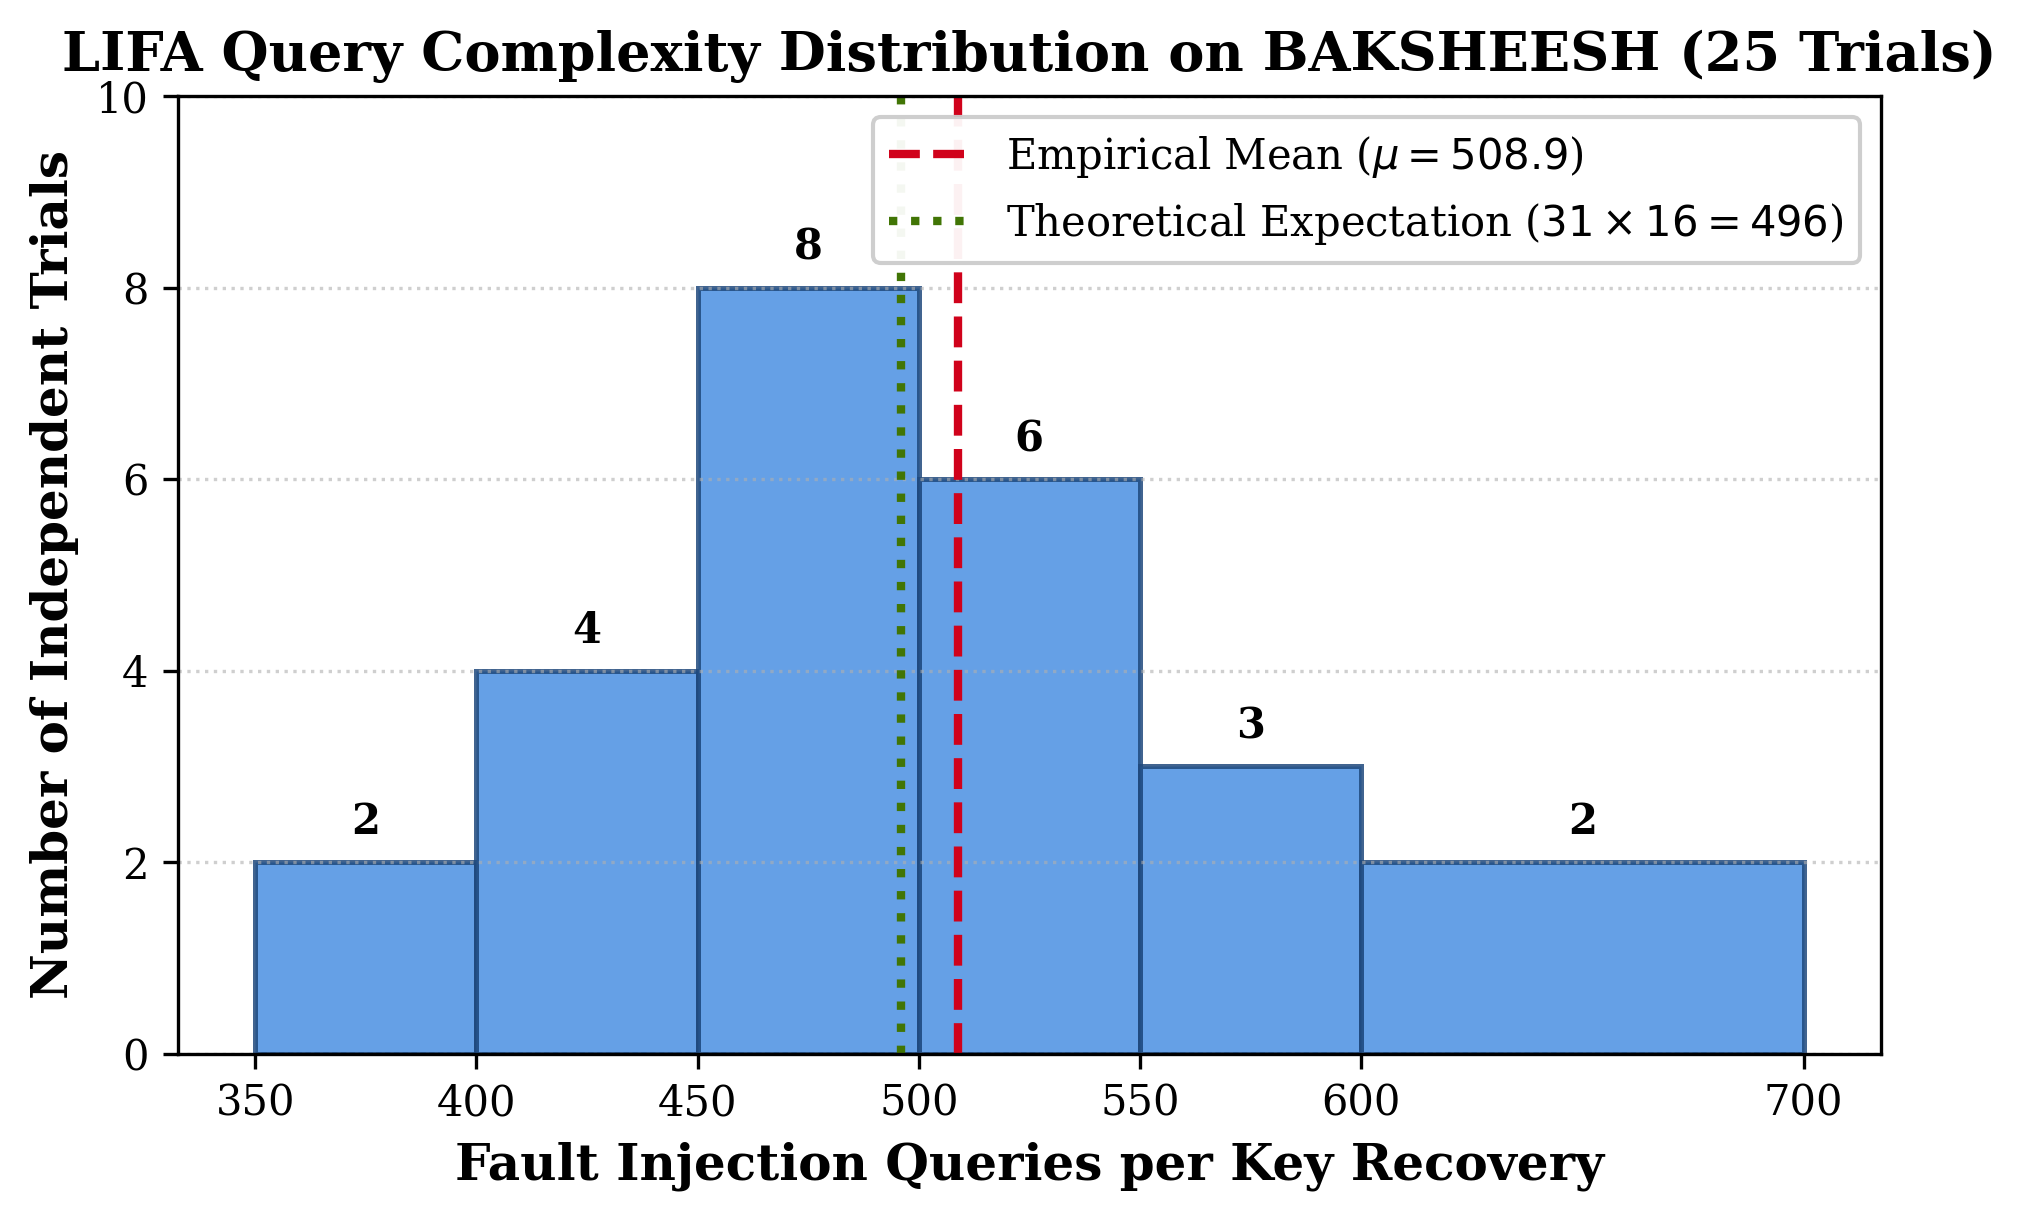
\includegraphics[width=\linewidth]{figures/fig4_lifa_histogram.png}
\caption{LIFA query distribution (25 trials, $\mu = 508.9$).}
\label{fig:lifa_hist}
\end{minipage}\hfill
\begin{minipage}{0.42\linewidth}
\centering
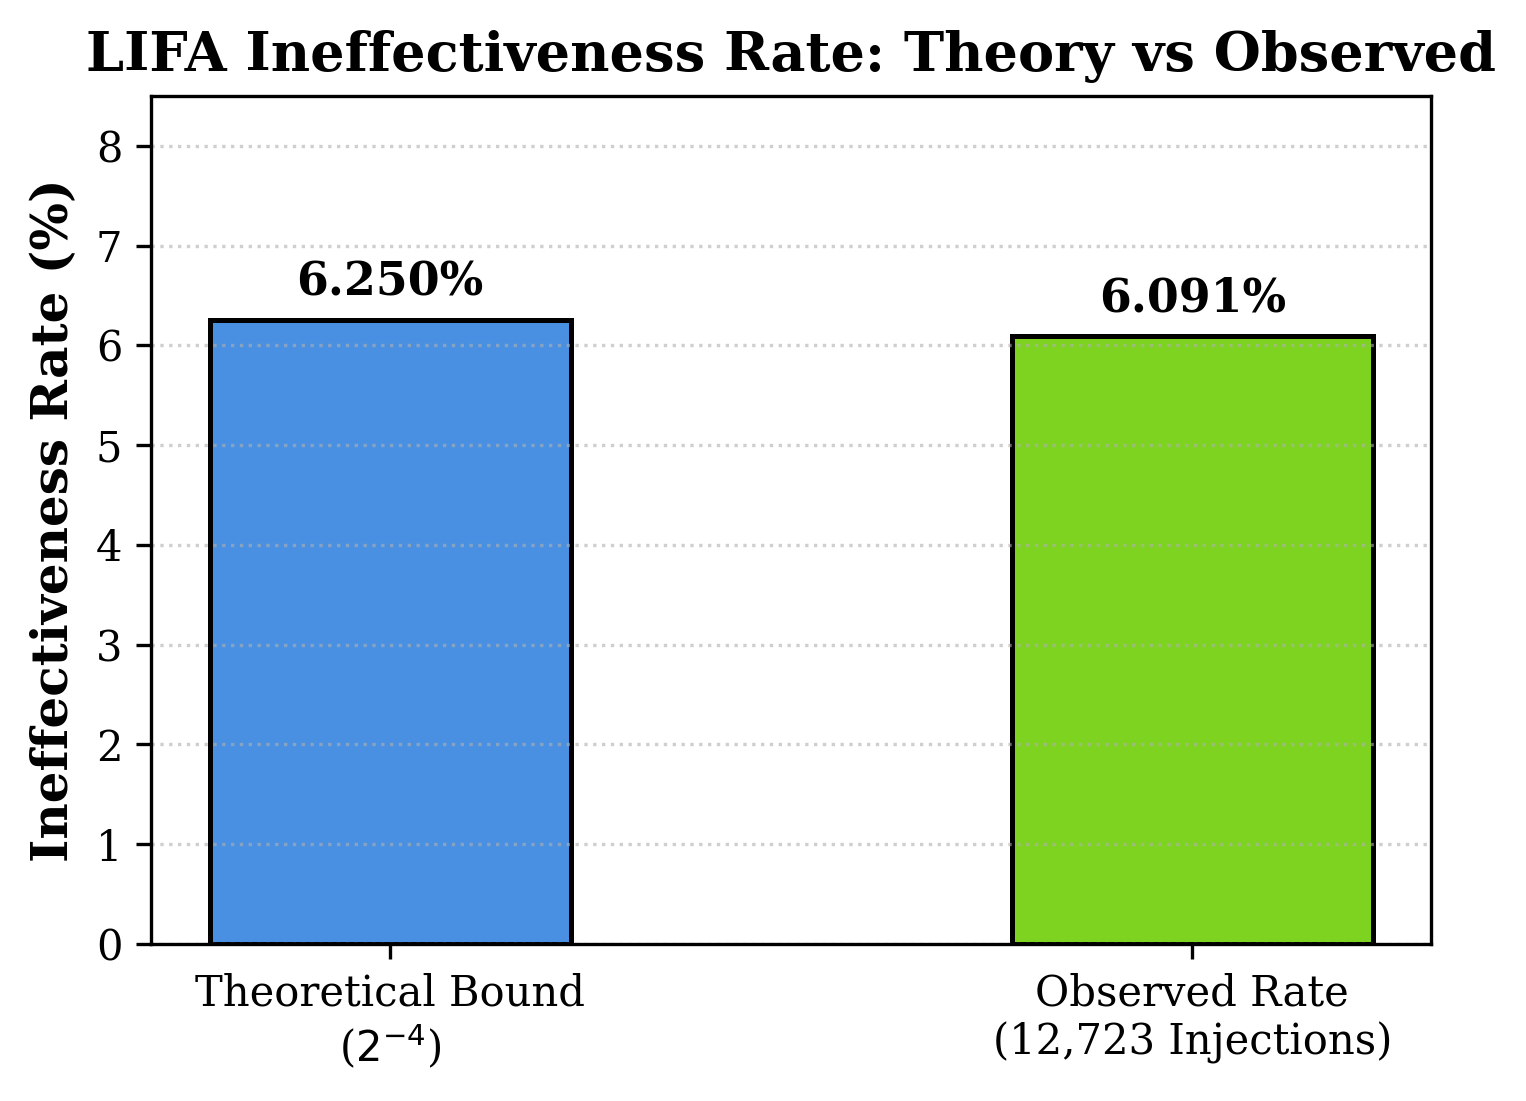
\includegraphics[width=\linewidth]{figures/fig5_ineffectiveness_rate.png}
\caption{Ineffectiveness rate: theory vs.\ observed.}
\label{fig:ineff_rate}
\end{minipage}
\end{figure}

\section{Unknown Fault Location Discovery Engine}
\label{sec:unknown_location_results}
In realistic physical attacks, the adversary does not know which of the $\binom{32}{2} = 496$ candidate pairs was hit by the glitch. We evaluated our blind identification engine across $N \in \{2, 3, 4, 5, 6, 8\}$ blind ciphertexts over 30 independent trials each:

\begin{table}[!htbp]
\centering
\caption{Unknown Fault Location Identification Accuracy vs. Ciphertexts ($N$).}
\label{tab:unknown_location}
\begin{tabular}{ccccc}
\toprule
\textbf{Ciphertexts ($N$)} & \textbf{Pairs Tested} & \textbf{Correct Identifications} & \textbf{Accuracy (\%)} & \textbf{False Match Rate ($496 \times 16^{-(N-1)}$)} \\
\midrule
2 & 30 & 0 & 0.0\% & $3.10 \times 10^1$ (Noise dominated) \\
3 & 30 & 14 & 46.7\% & $1.94 \times 10^0$ \\
4 & 30 & 28 & 93.3\% & $1.21 \times 10^{-1}$ \\
\textbf{5} & \textbf{30} & \textbf{30} & \textbf{100.0\%} & \textbf{$7.57 \times 10^{-3}$ ($< 0.8\%$)} \\
6 & 30 & 30 & 100.0\% & $4.73 \times 10^{-4}$ ($< 0.05\%$) \\
8 & 30 & 30 & 100.0\% & $1.85 \times 10^{-6}$ (Near-zero) \\
\bottomrule
\end{tabular}
\end{table}

\begin{figure}[!htbp]
\centering
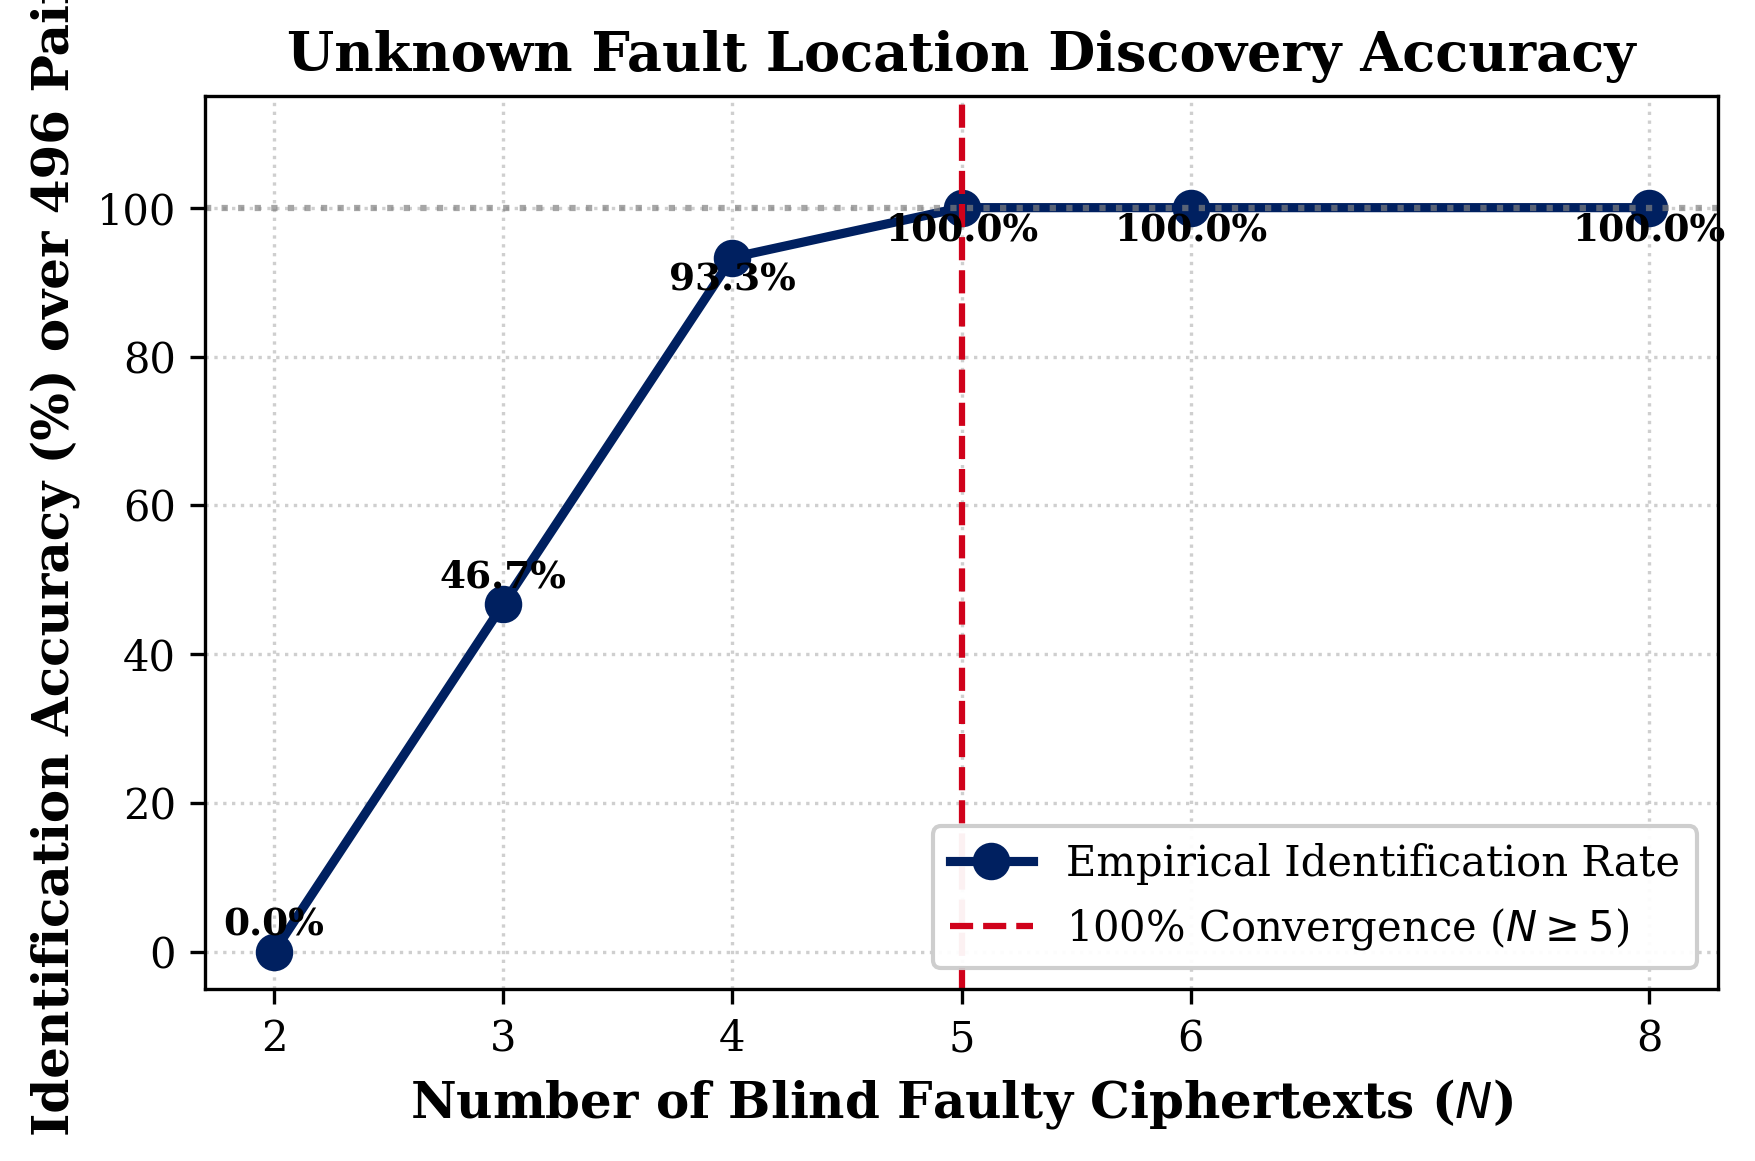
\includegraphics[width=0.65\linewidth]{figures/fig7_unknown_location_curve.png}
\caption{Unknown fault location discovery accuracy across 496 candidate pairs, achieving 100\% convergence at $N \ge 5$.}
\label{fig:unknown_loc_curve}
\end{figure}

\section{Noise Robustness and Missed Fault Tolerance}
\label{sec:noise_results}
Under physical glitch channels with miss rate $p_{\text{miss}} \in [0\%, 40\%]$, majority voting over $N = 30$ attempts per relation achieves \textbf{100.0\% full 128-bit key recovery} across all tested noise levels up to $p_{\text{miss}} = 30\%$ (and even $40\%$), as shown in Figure~\ref{fig:noise_curve}.

\begin{figure}[!htbp]
\centering
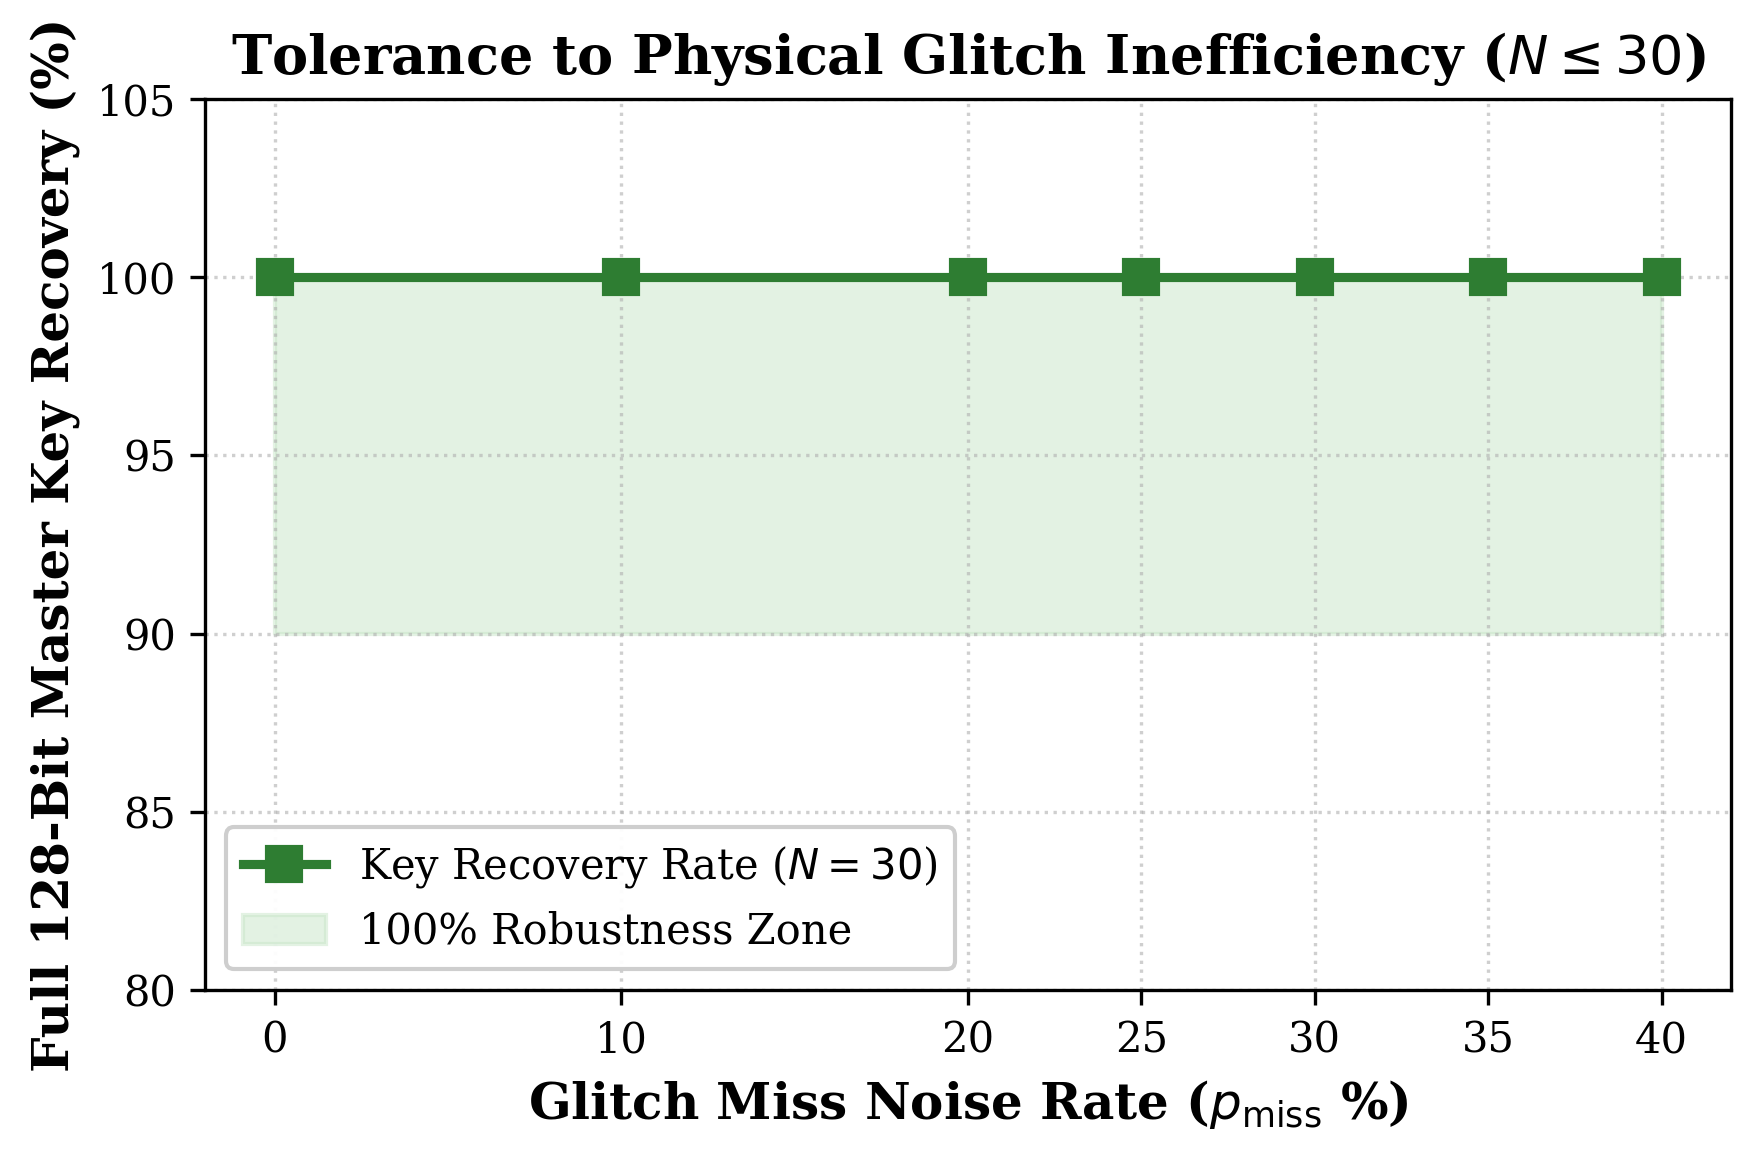
\includegraphics[width=0.65\linewidth]{figures/fig8_noise_tolerance_curve.png}
\caption{Full 128-bit master key recovery success rate under physical glitch miss noise ($p_{\text{miss}} \le 40\%$).}
\label{fig:noise_curve}
\end{figure}

\section{Comparative Evaluation: BAKSHEESH vs. GIFT-128}
\label{sec:baksheesh_vs_gift_results}
Figure~\ref{fig:bk_vs_gift} and Table~\ref{tab:comparison_summary} compare the empirical performance of BAKSHEESH and GIFT-128 under Linked Fault Analysis.

\begin{figure}[!htbp]
\centering
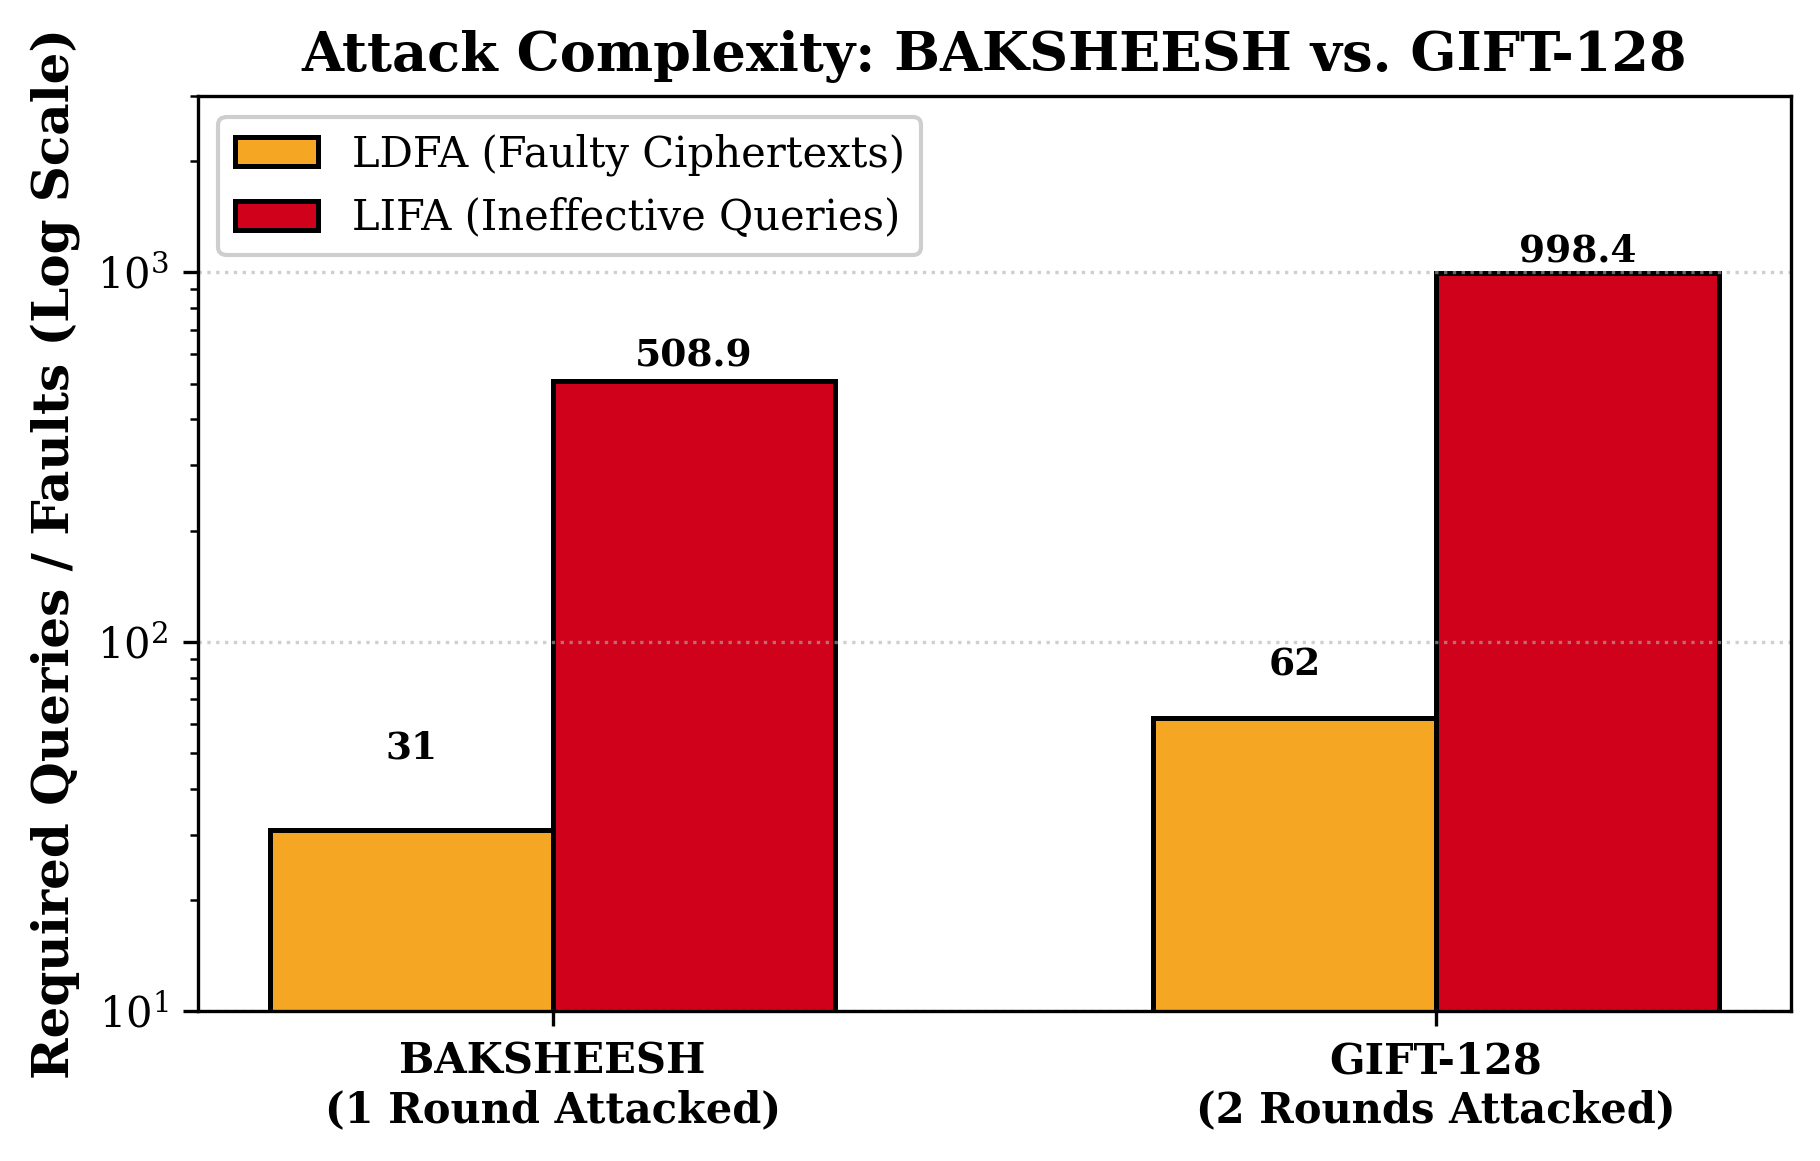
\includegraphics[width=0.68\linewidth]{figures/fig6_baksheesh_vs_gift.png}
\caption{Comparative query complexity of BAKSHEESH vs. GIFT-128 under LDFA and LIFA (log scale).}
\label{fig:bk_vs_gift}
\end{figure}

\begin{table}[!htbp]
\centering
\caption{Comprehensive Comparison: BAKSHEESH vs. GIFT-128 under LFA.}
\label{tab:comparison_summary}
\begin{tabular}{lccc}
\toprule
\textbf{Metric} & \textbf{BAKSHEESH} & \textbf{GIFT-128} & \textbf{Ratio (GIFT / BAKSHEESH)} \\
\midrule
Attacked Rounds & 1 (Round 35) & 2 (Rounds 39 \& 40) & $2.0\times$ \\
Key Injection Width & 128 bits / round & 64 bits / round & $0.5\times$ \\
LDFA Fault Injections & 31 & 62 & $2.0\times$ harder on GIFT \\
LIFA Mean Attack Queries & 508.9 & 998.4 & $1.96\times$ harder on GIFT \\
Theoretical Query Bound & $31 \times 16 = 496$ & $62 \times 64 = 3,968$ & $8.0\times$ higher bound \\
Candidate Keys Left & 16 ($2^4$) & 256 ($2^8$) & $16.0\times$ search on GIFT \\
Key Recovery Success Rate & 100\% (25/25) & 100\% (10/10) & Both Fully Broken \\
\bottomrule
\end{tabular}
\end{table}
